\chapter{IEC 61499 Function Block Standard}
\label{functionblocks}

\begin{bf}
{This chapter is with minor revisions copied from chapter 2 in \cite{j:des:2002}.}
\end{bf}

New technologies and standards are emerging that are set to
have a dramatic effect on the design and implementation of
industrial control systems. A new standard
IEC-61131-3~\cite{iec:1131:1993} was introduced in 1995 to
standardize the representation of control designs so as to
enable cross-vendor integration. The standard offered
significant advantages over earlier vendor proprietary
control design representations~\cite{l:pro:1995}.
\begin{itemize}
\item It encouraged well-structured procedural programs that
  allowed the development of different functional elements
  into separate procedures or program units.
\item It provided standardized languages and methods of
  program execution so that wide range of technological
  problems can be programmed as vendor-independent software
  elements.
\item It provided support for various languages like
  structured text, function block diagrams, ladder diagrams,
  instruction list and sequential function charts.
\item The standard enforced strong data typing and supported
  user defined data structures.
\end{itemize}

The standard however was based on a scanning mechanism where the
program execution was monitored by a continuous loop. Although
different parts of the program could be scanned at different
frequencies (based on fidelity requirements), it was tedious to
describe such behavior using sequential function charts. The
standard was based on polling mechanism rather than an event
driven system, and hence its execution order is not clearly
defined.

Further the standard was designed to support a software model and
languages for PLCs whose software was typically running on a
single processing resource. The communication between different
resources was supported through global variables and communication
blocks, both of which did not provide a clear and concise method
for defining the connections between distributed systems.

To overcome these problems, a function block model was sought that
would support distributed control systems in a scalable,
extensible and flexible manner. IEC-61499~\cite{iec:61499:2000}
standard has now been developed for distributed industrial
process, measurement and control systems.

In industrial systems, function blocks are now an established
concept for defining robust, re-usable software components. A {\it
Function Block} instance is defined to a software function unit
comprising an individual, named copy of a data structure and
associated operations specified by a corresponding function type.

Function blocks are analogous to objects in object-oriented
programming. Control designers can now take standard proven
encapsulated functionality in the form of blocks and link it
together in the quickest and most intuitive way possible. They
reduce the complexity since system integrators can now build large
systems using {\it black-box composition} i.e. without worrying
about how the internals of a block work.

The following sections are adapted largely from the various
discussions on the features of the standard in ~\cite{iec:61499:2000,
iec:1131:1993, l:pro:1995, l:mod:2001, c:des:2002, c:ope:2002}

\section{Reference Models}
IEC-61499 has provided a set of models for describing distributed
systems that have been programmed using function blocks.
\begin{itemize}
\item {\bf System Model:} At the physical level, a distributed
system consists of a set of co-operating {\it applications}. An
application can exist on a single system such as application C in
figure \ref{f:System_Model} or have functionality distributed over
a number of devices such as applications A and B in Figure
\ref{f:System_Model}.

\item {\bf Device Model:} A resource provides independent
execution and control of networks of function blocks. It supports
zero or more {\it resources} and has at least one interface. The
interface could either be a 'process interface' that allows the
resources to exchange data with the input and output points on the
physical devices, or a communication interface that allows the
resources to communicate with external resources in remote
devices. The device model is illustrated in Figure
\ref{f:Device_Model}.


\item {\bf Resource Model:} A resource is an independent functional unit,
contained in a device which has independent control of its
operation. The resource can be created, configured, parameterized,
started up, deleted etc. without effecting other resources. Each
resource provides an interface to the communication systems and
tot the device specific process. The resource is therefore,
concerned with the mapping of data and event flows which pass
between function blocks in the local resource to remove resource
function blocks via the device communication interfaces.

Figure \ref{f:Resource_Model} depicts the main features of an IEC
61499 resource. Within the resource, it shows a network of
interconnected function blocks linked by data and event flows. A
scheduling function ensures that the events are executed in the
correct serial order. {\it Service Interface} function blocks are
a special form of function blocks that provide a link between
function blocks and the interface of the resource.

\item {\bf Application Model:} An application is defined as a
network of interconnected function blocks, linked by data and
event flows. An application can be fragmented and distributed over
many resources. The resources ensure that the events are executed
in the correct serial order based on the causal relationships
specified by the applications.

An application could be understood as an entire set of function
blocks and interconnections to solve a particular automation
control problem. Figure \ref{f:Application_Model} illustrates an
application, where each individual block is either a function
block or a subapplication.

\item {\bf Function Block Model:} A function block is a functional
unit of software that its own data structure which can be
manipulated by one or more algorithms. The formal description of
the data structure is provided by the function block type
definition.

The main features of function blocks are:
\begin{itemize}
\item Each function block has a type name and an instance name.
\item Each block ha a set of event inputs, which can receive
inputs from other blocks through event connections.
\item Each block has one or more outputs, through which it can
propagate its results to other blocks.
\item There is a set of data inputs that allow values to be passed
in from other blocks.
\item There is a set of data outputs, through which the block can
pass its results to other blocks.
\item Each block may have a set of internal variables that hold
its state between algorithm invocations.
\item The behavior of the block is defined in terms of algorithms
and state information. This behavior is defined in the function
block type definition.
\end{itemize}

Figure \ref{f:Function_Block_Char} shows the main characteristics
of a function block. The top part of the block, called the
'execution control' portion contains in some cases, a state
machine that maps events to the algorithms that should be
triggered as a consequence of the event. The lower portion of
block contains both the algorithms and the internal data, both of
which are encapsulated within the block.

\end{itemize}

%
%%\singlespace
\begin{figure}
\begin{center}
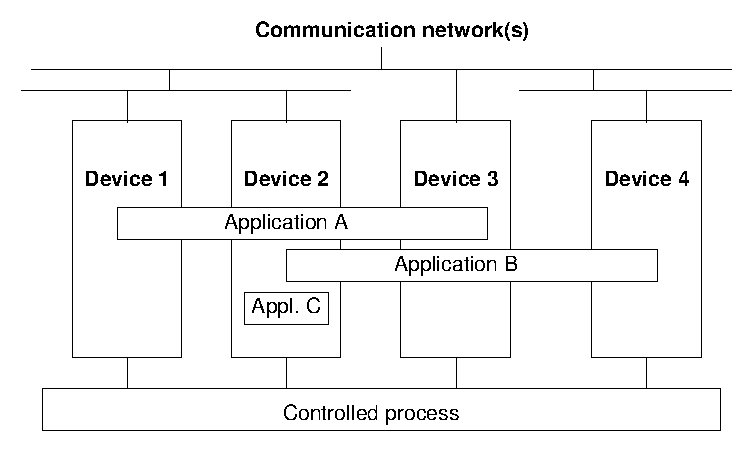
\epsfig{file=images/functionblocks/System_Model.eps, scale=.8} \caption[System
Model]{System Model {\protect ~\cite{iec:61499:2000}}}
\label{f:System_Model}
\end{center}
\end{figure}
%%\doublespace
%

%
%%\singlespace
\begin{figure}
\begin{center}
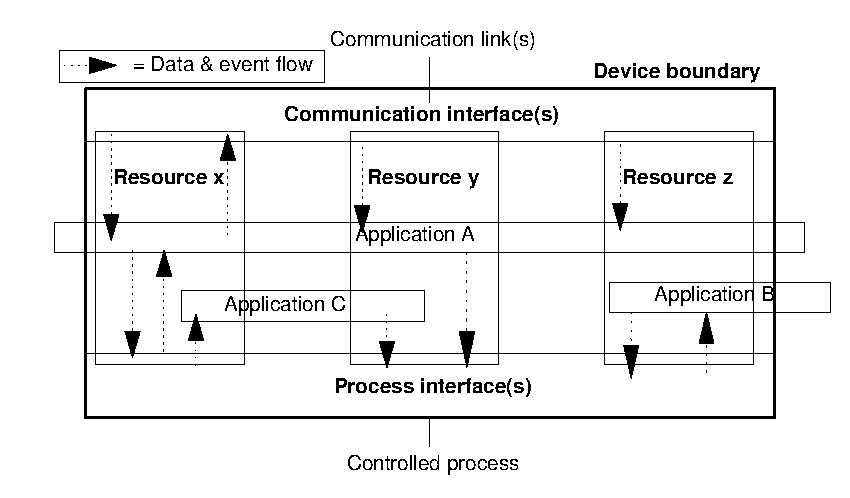
\epsfig{file=images/functionblocks/Device_Model.eps, scale=.8} \caption[Device
Model]{Device Model{\protect ~\cite{iec:61499:2000}}}
\label{f:Device_Model}
\end{center}
\end{figure}
%%\doublespace
%

%
%%\singlespace
\begin{figure}
\begin{center}
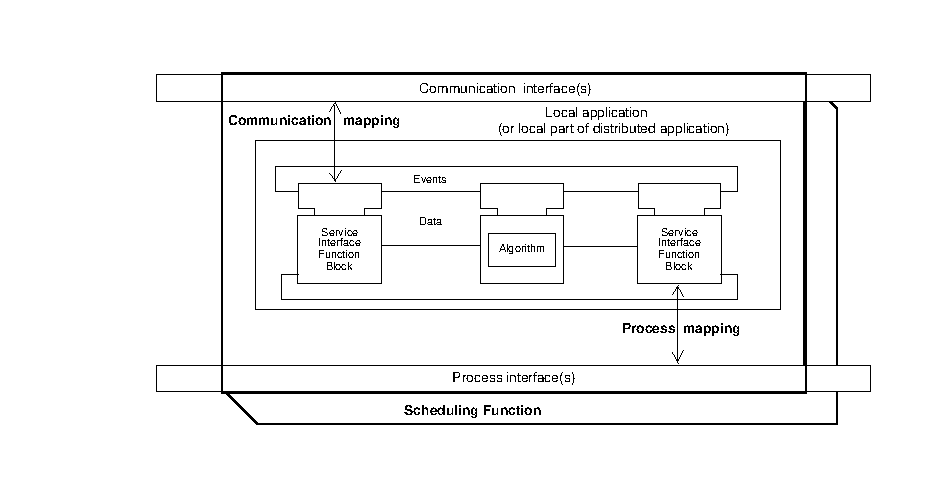
\epsfig{file=images/functionblocks/Resource_Model.eps, scale=.8} \caption[Resource
Model]{Resource Model{\protect ~\cite{iec:61499:2000}}}
\label{f:Resource_Model}
\end{center}
\end{figure}
%%\doublespace
%

%
%%\singlespace
\begin{figure}
\begin{center}
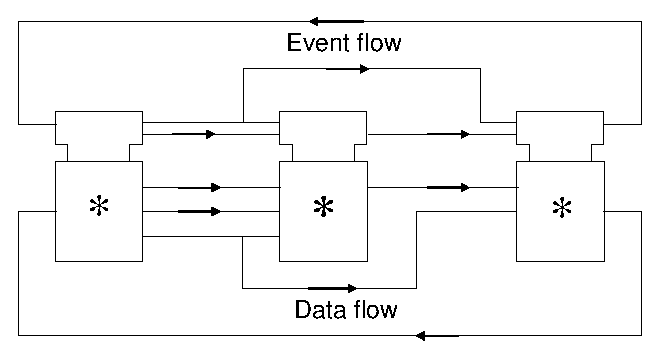
\epsfig{file=images/functionblocks/Application_Model.eps, scale=.8}
\caption[Application Model]{Application Model{\protect
~\cite{iec:61499:2000}}} \label{f:Application_Model}
\end{center}
\end{figure}
%%\doublespace
%

%
%%\singlespace
\begin{figure}
\begin{center}
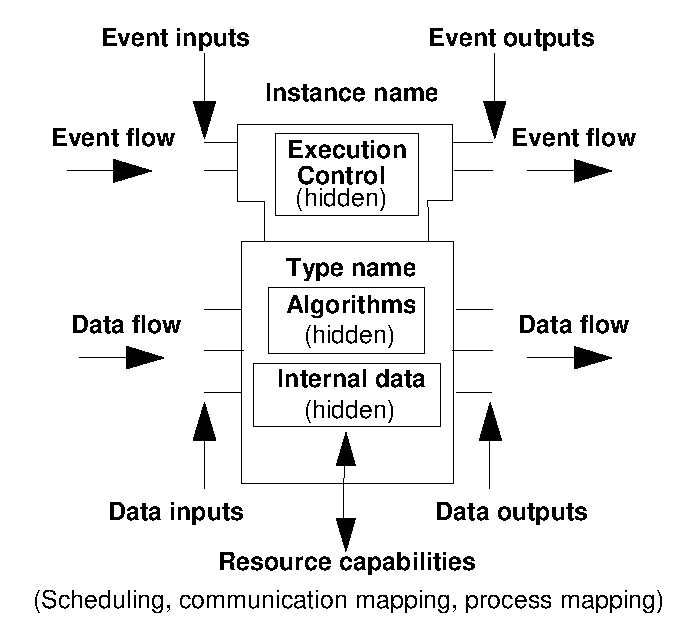
\epsfig{file=images/functionblocks/Function_Block_Char.eps, scale=.8}
\caption[Function Block Characteristics]{Function Block
Characteristics{\protect ~\cite{iec:61499:2000}}}
\label{f:Function_Block_Char}
\end{center}
\end{figure}
%%\doublespace
%

\section{Function Block Types}

A function block type is defined by a type name, formal
definitions for the input events and data and the output events
and data. The type definition also includes the internal behavior
of the block. The notion of a function block type is analogous to
the class definition in object-oriented programming while function
block instances correspond to the object instances of the classes.

\begin{itemize}
\item{\bf Basic Function Block Types:} The behavior of basic
function blocks is defined in terms of algorithms that are invoked
in response to input events. As algorithms execute, they trigger
output events to signal their state to other blocks. The basic
blocks hold their state in terms of internal variables. Basic
function blocks also can communicate their state using input and
output data variables.

The mapping of events onto algorithms is expressed using a state
transition notation known as execution control chart and is
described in the next section. Figure \ref{f:Basic_Block} shows an
example of a basic function block.

\item{\bf Composite Function Blocks:} The behavior of a composite
function block is described in terms of the event and data
connections between its component function blocks. A composite
function block can be used to hide the internal interactions
between the component blocks and presenting a simplified interface
for use by the outside world. A composite function block is
illustrated in Figure \ref{f:Composite_Block}.

\item {\bf Service Interface Function Blocks:} Service interface
function blocks provide an interface between the function block
domain and the external services. Since a service interface
function block is primarily concerned with data exchange, it is
defined using time sequence diagrams. Examples of service
interface function blocks are communication blocks for publishing
and subscribing over a network and management blocks for
dynamically creating component blocks and event connections.

\item {\bf Event Function Blocks:} Event function blocks are some
special basic function blocks defined in the standard to ease the
management of events. These blocks are used for control,
generation and detection of events and can be used by other
composite blocks. These blocks are defined using an execution
control chart or a time sequence diagram. These blocks can be
used, for instance, for the following purposes.
\begin{enumerate}
\item To split events to produce new events
\item To allow events to be merged.
\item To permit the propagation of certain events.
\item To select between two or more events.
\item To delay an event by a given period.
\item To generate a stream of events at a regular interval.
\end{enumerate}

\end{itemize}

%
%\singlespace
\begin{figure}
\begin{center}
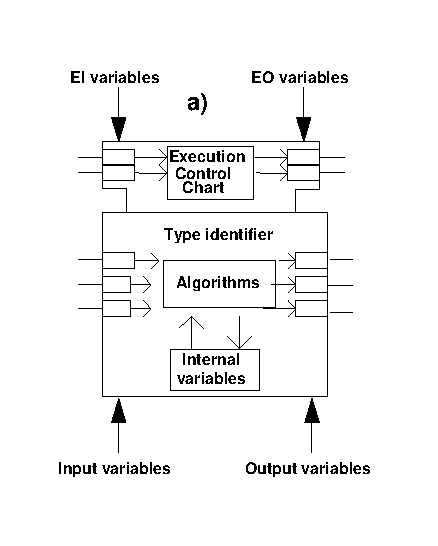
\epsfig{file=images/functionblocks/Basic_Function_Block.eps, scale=.8}
\caption[Basic Function Block]{Basic Function Block{\protect
~\cite{iec:61499:2000}}} \label{f:Basic_Block}
\end{center}
\end{figure}
%\doublespace
%

%
%\singlespace
\begin{figure}
\begin{center}
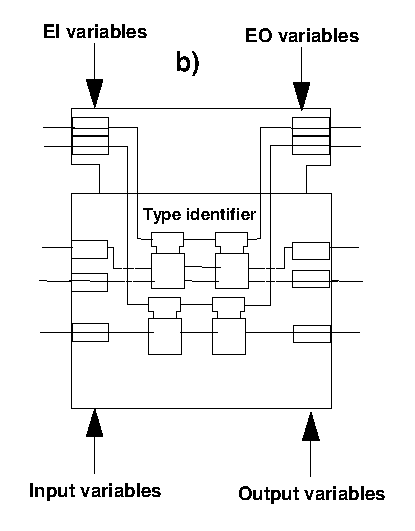
\epsfig{file=images/functionblocks/Composite_Function_Block.eps, scale=.8}
\caption[Composite Function Block]{Composite Function
Block{\protect ~\cite{iec:61499:2000}}} \label{f:Composite_Block}
\end{center}
\end{figure}
%\doublespace
%

\section{Execution Model}

The execution of algorithms for basic function blocks is invoked
by the execution control portion of a function block instance in
response to events at event inputs. This invocation takes the form
of a request to the underlying scheduling function of the
associated resource to schedule the execution of algorithm's
operations. The model assumes that the resource in which a
function block exists provides a scheduling function that ensures
each phase of function block execution occurs in the correct order
and with the correct priority.

The execution model specifies eight discrete timing points as
shown in Figure \ref{f:Execution_Model} that must occur
sequentially for the basic function block to operate. These are:

\begin{description}
\item[$t_1$]: Values coming from external function blocks
as input data are stable at the current block.
\item[$t_2$]: The event associated with the input values occurs.
\item[$t_3$]: The execution control function notifies the resource
scheduling function that it has the input values and is ready to
execute the algorithm.
\item[$t_4$]: The scheduling function begins the algorithm execution.
\item[$t_5$]: The algorithm processes input values, (and in some
cases, internal variables) to create new output values that are
written to the block's outputs.
\item[$t_6$]: The algorithm notifies the scheduling function that it
has completed its execution.
\item[$t_7$]: The scheduling function invokes the execution control
to generate the output events.
\item[$t_8$]: The execution control generates the appropriate output
events at its event output ports. The event may be used by
downstream blocks to signal that they may use the output values
generated by this block.
\end{description}

%
%\singlespace
\begin{figure}
\begin{center}
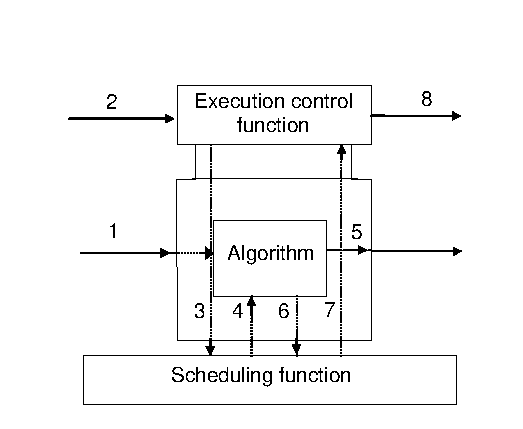
\epsfig{file=images/functionblocks/Execution_Control_Chart.eps, scale=.8}
\caption[Execution Model]{Execution Model{\protect
~\cite{iec:61499:2000}}} \label{f:Execution_Model}
\end{center}
\end{figure}
%\doublespace
%

To ensure consistency, the algorithms must use the snapshot of
input variables that exists when the input event arrived. Further
the scheduling function must be able to detect the arrival of
input events at a faster rate than the rate at which they can be
handled by the block.


% \section{FBEditor}
% Function Block Development Kit (FBDK) ~\cite{c:fun:2002} is a
% software toolkit that enables users to build and test data types,
% function block types, resource types, device types and system
% configurations according to the IEC 61499 standard. FBEditor is a
% part of the FBDK toolkit that provides a development and runtime
% environment for applications based on the IEC 61499 standard.
% Figure \ref{f:FBEditor} shows the editor being used to load a
% function block used for controlling a motor.

% %
% %\singlespace
% \begin{figure}
% \begin{center}
% \epsfig{file=images/functionblocks/FBEditor.eps, scale=.6}
% \caption[FBEditor]{FBEditor{\protect ~\cite{c:fun:2002}}}
% \label{f:FBEditor}
% \end{center}
% \end{figure}
% %\doublespace
% %

% FBEditor enables the users to edit the block definitions through
% both a text editor and through a graphical user interface. New
% data types, basic function blocks, composite function blocks,
% execution control charts and other higher level entities may be
% created through the editor. The attributes of the blocks (data and
% events) may also be examined through a graphical user interface.
% The function blocks can be examined at the device level as shown
% in Figure \ref{f:Editor-Devices} or at the level of individual
% attributes like the connections, as shown in figure
% \ref{f:Editor-Mapping}.

% The editor supports the languages supported by the standard
% (Structured text, execution control chart etc.). It uses XML as
% the exchange format to ensure portability across various domains.
% Figure \ref{f:Editor-Versions} shows how the editor can also be
% used to manage meta properties like versions, owner entities,
% authors etc.

% %
% %\singlespace
% \begin{figure}
% \begin{center}
% 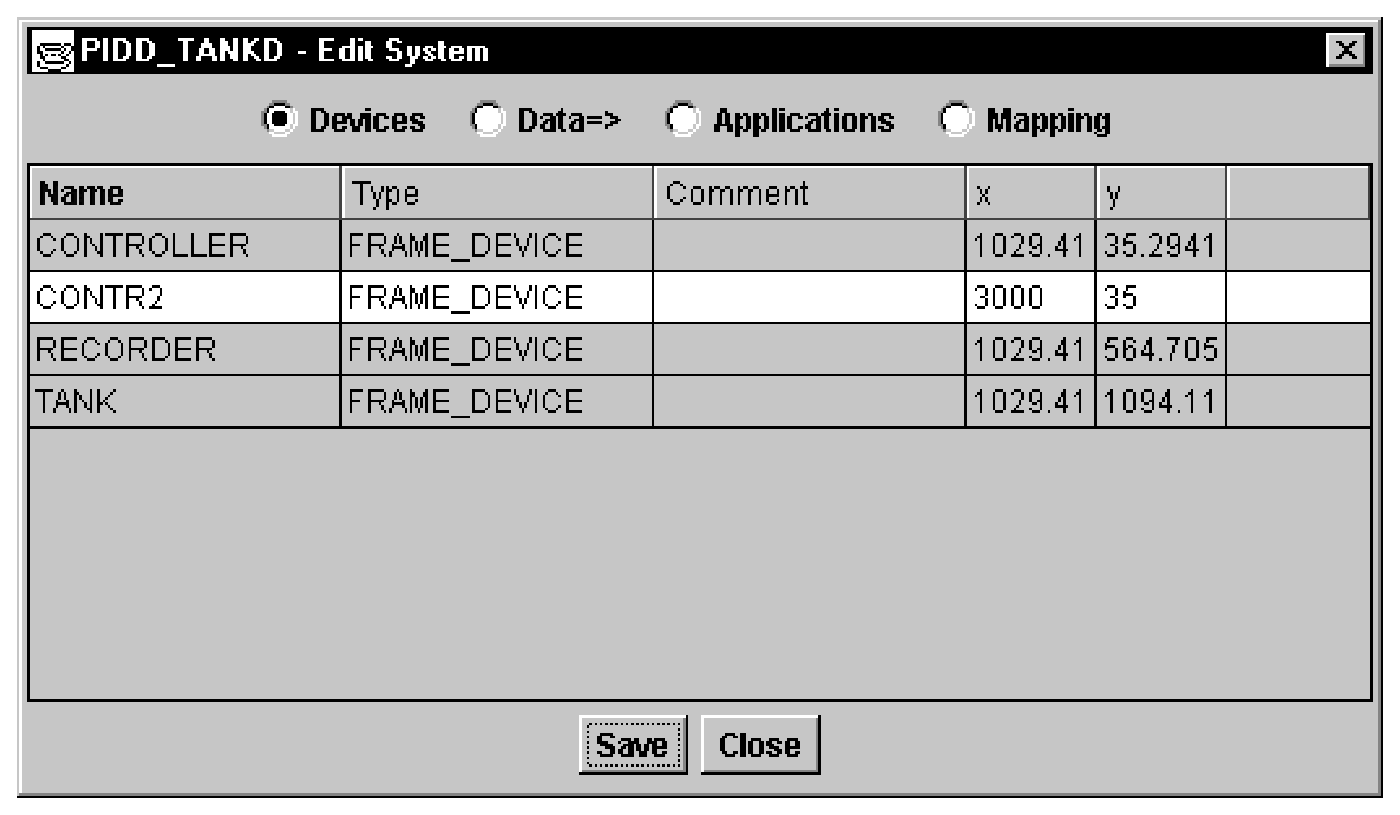
\epsfig{file=images/functionblocks/Editor-Devices.eps, scale=.6} \caption[FBEditor
% - Editing system devices]{FBEditor - Editing system
% devices{\protect ~\cite{c:fun:2002}}} \label{f:Editor-Devices}
% \end{center}
% \end{figure}
% %\doublespace
% %

% %
% %\singlespace
% \begin{figure}
% \begin{center}
% 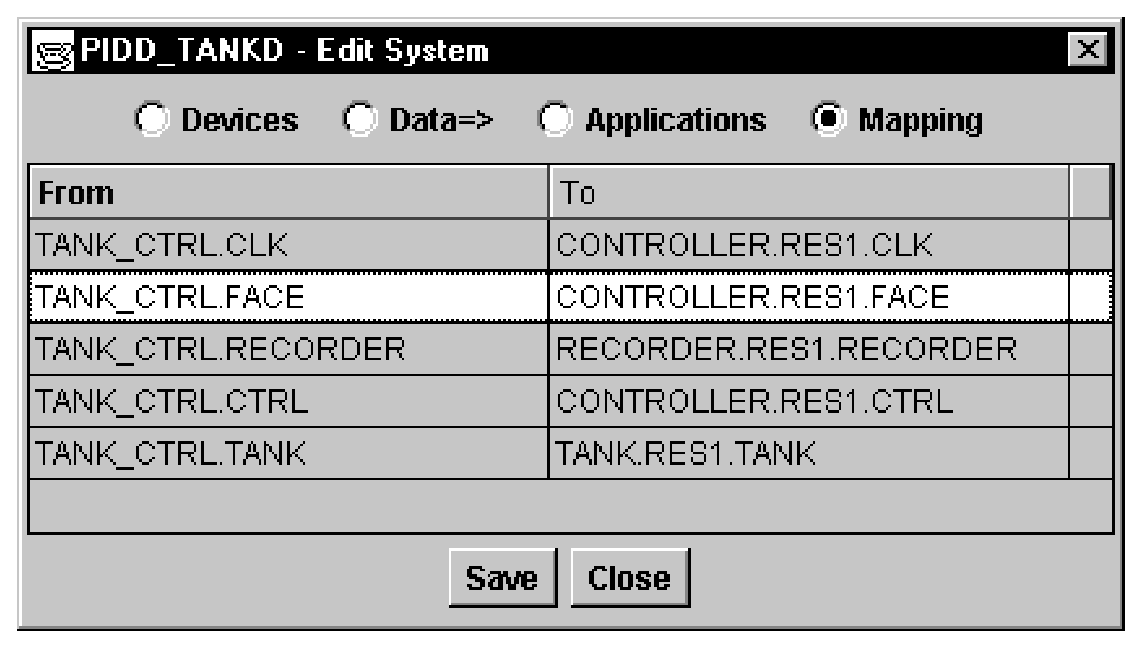
\epsfig{file=images/functionblocks/Editor-Mapping.eps, scale=.6} \caption[FBEditor
% - Editing device connections]{FBEditor - Editing device
% connections{\protect ~\cite{c:fun:2002}}} \label{f:Editor-Mapping}
% \end{center}
% \end{figure}
% %\doublespace
% %

% %
% %\singlespace
% \begin{figure}
% \begin{center}
% 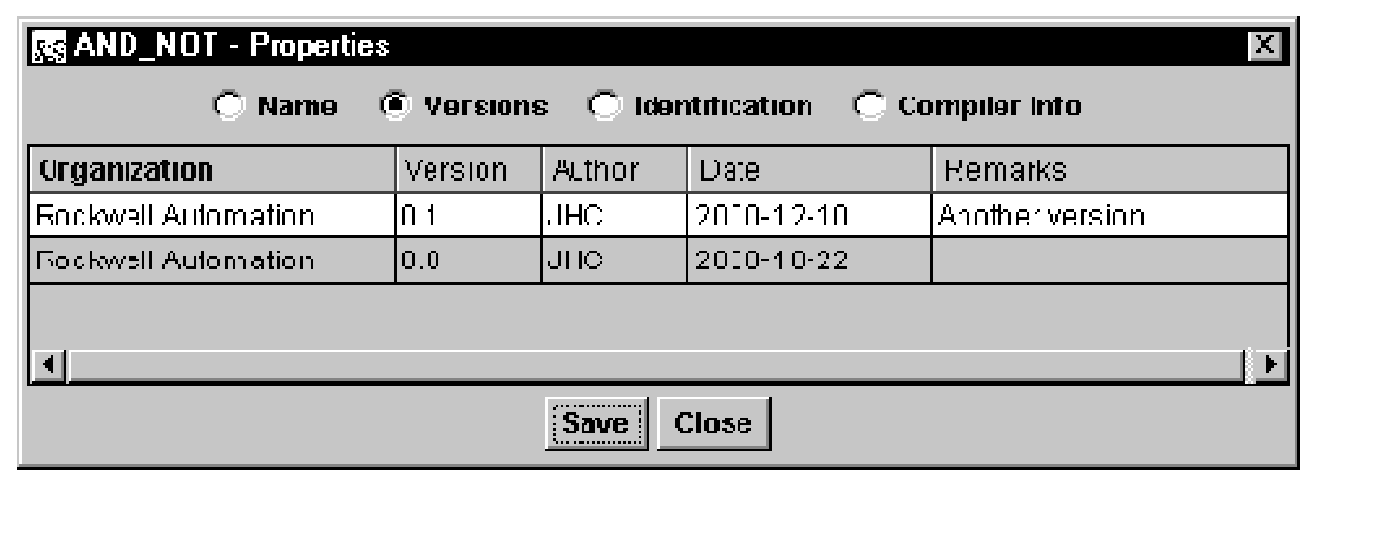
\epsfig{file=images/functionblocks/Editor-Versions.eps, scale=.6}
% \caption[FBEditor - Editing meta properties]{FBEditor - Editing
% meta properties{\protect ~\cite{c:fun:2002}}}
% \label{f:Editor-Versions}
% \end{center}
% \end{figure}
% %\doublespace
% %
% FBEditor has a navigation pane that allows the user to choose the
% display on the worksheet area, including the external interface;
% the Execution Control Chart (ECC) for basic function block type;
% service primitive sequences for service interface function block
% types; and function block networks for composite function block
% types, device and resource types and instances, and system
% configurations. The worksheet / viewport area contains the
% function block diagram for the currently selected instance.
% Different components of the diagram can be dragged around for
% better readability.


% FBEditor has been developed in Java language. Hence in order to
% run simulations on applications written using the editor, one
% needs to generate the Java classes that correspond to the source
% files for the function blocks written in structured text (for
% instance). The editor has a code generation mechanism through
% which it parses through the source files and generates a Java
% class corresponding to each block.


% On occurrence of certain input events, the user needs to specify
% the algorithms that should be scheduled to be executed and the
% output events that should signal the completion of algorithms.
% This may be done either by editing the generated Java files or by
% enclosing the algorithm inside especially marked tags in the
% source files. The files are then compiled and simulations can be
% run from within the editor environment. Figure
% \ref{f:Editor-Transitions} shows the assignment of output events
% on the transitions through the editing of the execution control
% chart.

% %
% %\singlespace
% \begin{figure}
% \begin{center}
% 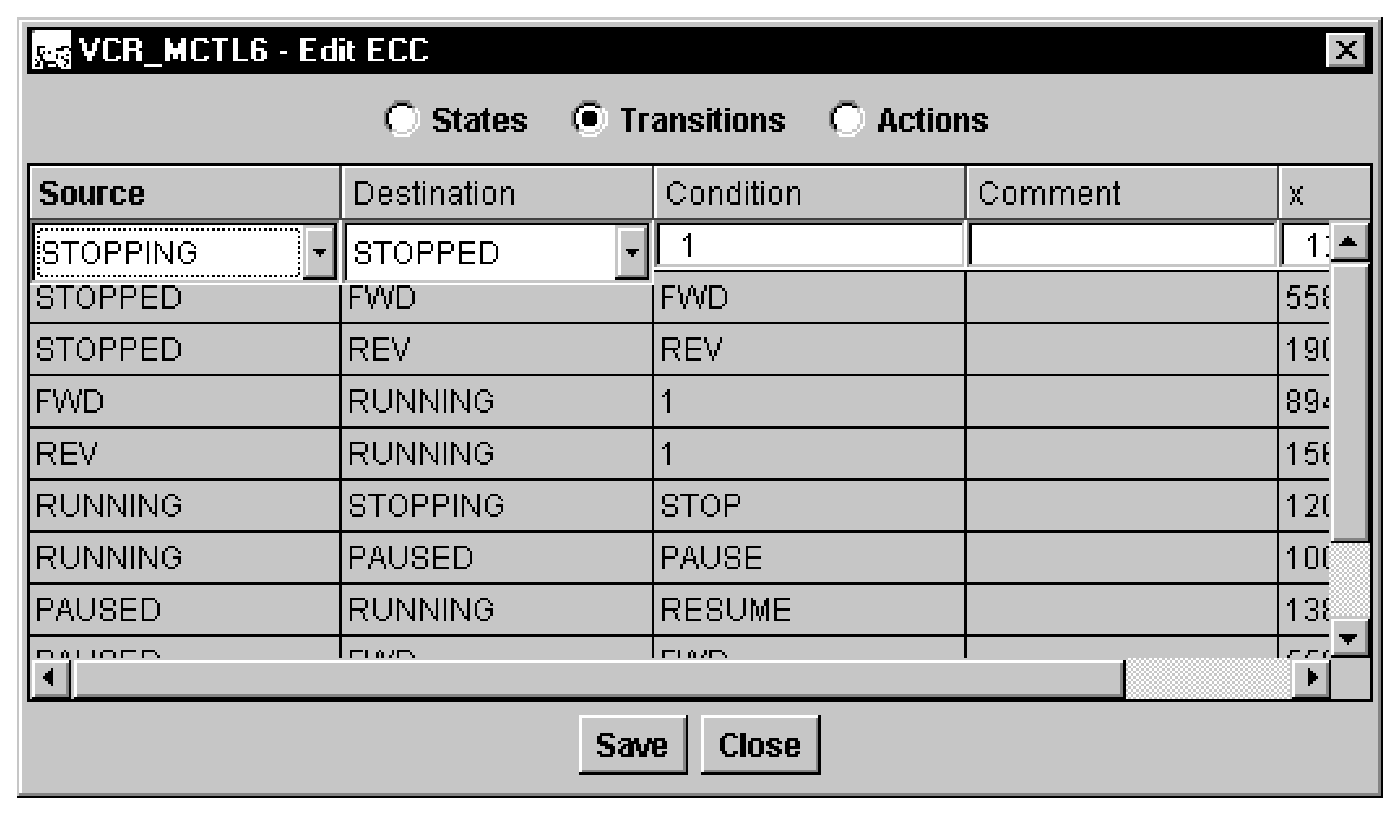
\epsfig{file=images/functionblocks/Editor-Transitions.eps, scale=.6}
% \caption[FBEditor Editing the execution control chart]{FBEditor
% Editing the execution control chart{\protect ~\cite{c:fun:2002}}}
% \label{f:Editor-Transitions}
% \end{center}
% \end{figure}

%\doublespace
%

%\section{EMBench and Function Blocks}

%Since the FBEditor provided the aforementioned functionality, it
%was decided that the EMBench should leverage it. In particular,
%the bench relies on the editor for two basic features.
%\begin{enumerate}
%\item To generate the Java files from the IEC 61499 source files.
%\item To manage the Java thread that initializes the blocks during
%simulation.
%\end{enumerate}

%It has been visualized that the bench will eventually have the
%editor as one of its components. The bench explicitly manages the
%design activities of the user and generates the function block
%definitions for the user design. It then requests the FBEditor
%component to load the specified source files, generate the Java
%classes and run the simulation. In addition, the user may make
%behavioral changes to the blocks by editing the events, if he/she
%so desires. The editor conforms to the published service
%specifications of the bench as explained in chapter \ref{chap3}
%and hence would present the same interface to the client.

%Currently, however, the FBEditor is not a part of the bench
%because it does not expose an API. Since it is external to the
%bench, the bench has to circumvent this problem by allowing the
%editor to be executed as a separate application and delegating the
%simulation task completely to the editor. The data exchange
%necessary between the two applications is handled via network
%communication. This issue is explained in a greater detail in
%chapter~\ref{chap4} and chapter~\ref{chap5}.
